\section{Overview of Pytheas Ideas}
\label{sec:pytheas:overview}

%In a general setting, the combination of the above challenges 
% might make \mab intractable. However, 
To address the practical challenges of applying \mab in network applications, 
we observe a key domain-specific insight in networked applications
 that enables us to address both challenges in practice. We highlight the intuition 
 behind our insight, which we refer to as \idea, and then provide an overview of the \name system 
 which builds on this insight.  

%called \idea, inspired by the insight that sessions with
%similar context are often nearby in terms of geographical location and IP
%space, and can be grouped.

\mypara{Insight of  \Idea}
Our insight is that the ``network context'' of application sessions is often aligned with
their ``network locality''.
That is, if two sessions share the context that determines their \mab decisions, 
they will be likely to match on some network-specific features.
We see manifestations of this insight in many settings.
% When clients share certain location or IP prefix-related
%features, they are more likely to have the similar video QoE~\cite{cfa} and
%similar TCP throughput~\cite{cs2p,spand} at the same point of time. 
 For instance, video
sessions with similar QoE from the same CDN/server tend to match on 
client IP prefix~\cite{cfa,cs2p}. 
Similarly, VoIP calls between the same ASes are likely to share the best
relays~\cite{via},  and clients from  same /24 IP prefix will have
similar web load time from the same edge proxy~\cite{footprint}.
In Section\ref{subsec:frontend}, we validate this insight with a real-world dataset.

%This insight suggests two natural implications:
%\begin{packeditemize}
%
%\item First, a global view is not necessary to run \mab for network applications.
%
%\item Second, when a session queries a frontend cluster for decision, the same cluster is likely to receive the data of other sessions in the same group.
%\vyas{this is still bad. the notion of frontend etc has not been defined!}
%
%\end{packeditemize}
%
%\vyas{there seems to be two insights --- group based ee can be done and these groups goto same frontend? but the 
% above insight doesnt imply they will get mapped to same frontend. also it might be cleaner to difrectly go below than this 
% indirect step}


%\begin{packeditemize}
%
%\item First, the \mab context of sessions has natural ``boundaries''.
%%\vyas{dont follow this cliff thing!}
%For instance, if two sessions share a performance bottleneck, they will be much more likely to share the same network context that affect their \mab decisions than otherwise. 
%In other words, it is not a necessary condition that \mab process needs a global view of QoE of all sessions.
%%We see such effect manifest itself in various applications, such as critical features in video streaming~\cite{cfa}, Internet telephony~\cite{via}, and web application sessions~\cite{??}.
%
%\item Second, sessions with similar \mab context are often in the same geographical locations and IP space.
%For instance, QoE of a video session is often critically determined by ASN~\cite{cfa}, which means video sessions sharing similar \mab context are likely in the same ASN.
%%Similar observations has also been made in TCP performance~\cite{spand}, Internet telephony~\cite{via}, and web application sessions~\cite{??}.
%
%\end{packeditemize}
%We see manifestations of both effects in a variety of applications.
%When clients share certain location or IP prefix-related features, they are more likely to have the similar video QoE~\cite{cfa} and similar TCP throughput~\cite{cs2p,spand} at the same point of time.
%Video sessions share similar QoE if the match location or IP prefix-related features~\cite{cfa}.
%Two Internet telephony calls are likely to share the best relay option when they have the same peering points with the relay services~\cite{via}.
%Users with same /24 IP prefix are very likely to have similar web load time from the same proxy or data center~\cite{footprint}.


This insight inspires the notion  of {\em \idea}, which can 
 address the above challenges by enabling an effective decomposition 
 of the \mab process (Figure~\ref{fig:system-overview}a).  
 Specifically, instead of a global \mab
process over all sessions, we group together sessions with similar context by 
network locality and other key features (such as device and location), and
use one \mab process for each group.
% It addresses the challenges of real-time
%\mab for two reasons:
%\begin{packeditemize}
%\item 
Since sessions within a group share network locality (e.g., 
in the same locations and IP prefixes), 
they are likely to be mapped to the same frontend cluster.
By running the per-group \mab logic in this frontend cluster, we can update
decisions with fresh data from other sessions in the group received by this frontend cluster.
%\item 
 Furthermore, as each group consists of sessions with similar context, 
it is sufficient to use traditional \mab techniques based on the data of sessions
in one group, 
without needing a global view of all sessions.
%\end{packeditemize}
It is important to note that sessions are not grouped entirely based on IP prefixes. The sessions in the same network locality could have very different QoE, depending on the device, last-hop connectivity, and other features. Therefore, we group sessions on a finer granularity than IP prefix.

\begin{figure}[t!]
\centering
%\includegraphics[width=0.5\textwidth]{figures/system-overview.pdf}
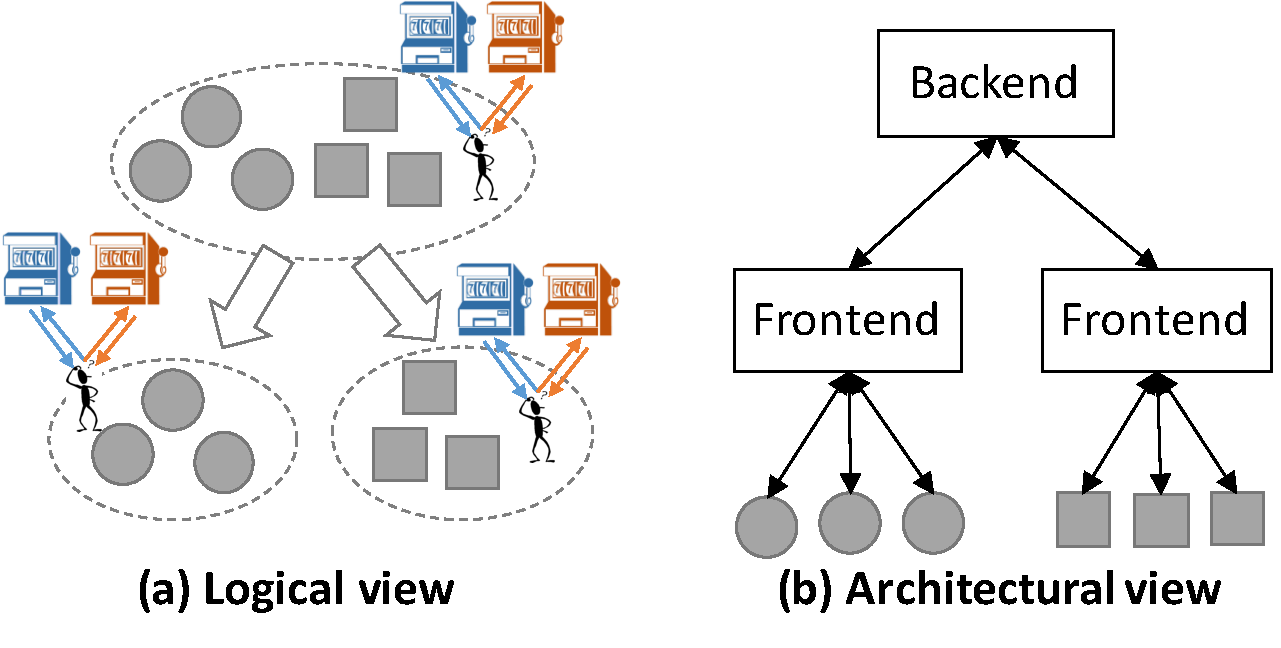
\includegraphics[width=0.6\textwidth]{figures/pytheas-system-overview-group.pdf}
%\vspace{-0.4cm}
\caption{Illustration of \idea.}
%\vspace{0.1cm}
\label{fig:system-overview}
\end{figure}



\mypara{System overview}
Figure~\ref{fig:system-overview}b shows how the \idea is realized in the \name architecture.
Each session group is managed
by one per-group \mab process run by one frontend cluster.  When a session
comes in, it sends a request for its control decisions, which includes its features,
to the \name system.  The request will be received by a frontend
cluster, which maps the session to a group based on its features, then
gets the  most up-to-date decision from the local per-group \mab process, and
returns the decision to the session.  Each  session measures its QoE and reports it  to the same frontend cluster.  When this frontend
receives the QoE measurement, it again maps the session to a group, and
updates the \mab logic of the group with the new measurement.  
In most cases, the
\mab logic of a group is run by the same cluster that 
receives the requests and
measurements of its sessions, 
so \mab logic can be updated in real time. 

%When the frontend cluster receives the control requests from another session
%in the same group, it returns the fresh decision made by the local \mab
%process.
%Nonetheless, when sessions of a group  are received by different clusters 
%(e.g., the ``square'' sessions in Figure~\ref{fig:system-overview}b), one of
%them will be picked to run the per-group \mab logic, and other clusters will
%cache the decisions and forward QoE measurements in a near real-time
%fashion.

%Note that multiple \mab processes can run in the same frontend cluster, and one group can span across multiple frontend clusters. 

 The backend cluster has a global, but
slightly stale, view of QoE of all sessions, and it determines the session
groups -- which group each session belongs to and which frontend should run
the per-group logic for each group.  Normally, such grouping is updated
periodically on a timescale of minutes. During sudden changes such as frontend cluster failures, it can also be triggered on demand to re-assign groups to frontend clusters.

%\camera{On a high level, group-based \mab addresses the challenges of applying \mab in network applications through (1) modeling ``network context'' by grouping session sharing QoE-determining factors, and (2) realizing real-time \mab by running control logic in the frontend clusters while learning the slow changing session groups in the backend cluster.}

The following sections will present the algorithms (Section~\ref{sec:pytheas:algo}) and system design (Section~\ref{sec:pytheas:system}) of \name, and how we implemented it (Section~\ref{sec:pytheas:impl}) in more details.


%\subsection{Running example}
%
%This part gives a simple running example to show the workflow of \name.


